\documentclass{article}[11pt]

\usepackage{amsmath}
\usepackage{amssymb}
\usepackage{nicefrac}

\usepackage{pdflscape}

\usepackage{upgreek}

\usepackage{bashful}

% No intendation
\setlength\parindent{0pt}

\usepackage{hyperref}

\usepackage{siunitx}
\sisetup{
  per-mode=fraction,
  fraction-function=\tfrac
}

\usepackage{listings}
  \lstset{
    basicstyle=\ttfamily,
    escapeinside=||,
    xleftmargin=1cm
  }

\usepackage{float}

\usepackage{longtable}

\usepackage{multirow}

\usepackage{tikz}
  \usetikzlibrary{patterns}
  \usetikzlibrary{arrows.meta}
  \usetikzlibrary{shapes.misc}
  \usetikzlibrary{calc}

\usepackage{pgfplots}

\usepackage{cleveref}
\crefmultiformat{equation}{(#2#1#3)}{ and~(#2#1#3)}{, (#2#1#3)}{ and~(#2#1#3)}


\usepackage{acronym}
\usepackage[acronym,nonumberlist]{glossaries}
\glsdisablehyper
\makeglossaries
\newacronym{spice}{SPICE}{Simulation Program with Integrated Circuit Emphasis}
\newacronym{lef}{LEF}{Library Exchange Format}
\newacronym{dft}{DFT}{Discrete Fourier Transform}
\newacronym{dtft}{DTFT}{Discrete-Time Fourier Transform}
\newacronym{fft}{FFT}{Fast Fourier Transform}
\newacronym{mosfet}{MOSFET}{Metal–Oxide–Semiconductor Field-Effect Transistor}
\newacronym{clm}{CLM}{Channel Length Modulation}
\newacronym{de}{DE}{differential equation}
\newacronym{soi}{SOI}{silicon-on-insulator}
\newacronym{ldo}{LDO}{low-dropout regulator}
\newacronym{ota}{OTA}{operational-transconductance amplifier}
\newacronym{ofa}{OFA}{operational-floating amplifier}

% literature
\usepackage[ backend=biber
           , isbn=true
           , sorting=none
           , style=ieee
           ]{biblatex}
\addbibresource{./../../literature.bib}

% definitions
\def \whatis       {Notes}
\def \title        {Fuubar}

\def \author       {Matthias Schweikardt}

\def \authorMail   {mschweikardt@posteo.de}

\def \authorGithub {mschweikardt}

\def \license      {CC BY-SA 4.0}
\def \licenseUrl   {https://creativecommons.org/licenses/by-sa/4.0/}

\def \date         {nodate}

\def \pdfurl       {https://mschweikardt.github.io/ee-notes/%
\bash[stdout]
IFS=/ 
var=($PWD)
echo ${var[-1]}
\END%
.pdf
}
\def \srcurl       {srcurl}


% Customize footer and header of document
\usepackage{fancyhdr}

% Access last page number
\usepackage{lastpage}

% Access last page number
\usepackage[thinc]{esdiff}

% Physics
\usepackage{physics}

% Comment environment
\usepackage{comment}

% Subcaptions
\usepackage{subcaption}

% Thicker lines in tables
\usepackage{booktabs}

% Indentation in footnote
\makeatletter
\renewcommand\@makefntext[1]{\leftskip=2em\hskip-0.5em\@makefnmark#1}
\makeatother         

% qty with the siunitx definition
\AtBeginDocument{\RenewCommandCopy\qty\SI}

% TikZ compatibility
\pgfplotsset{compat=1.18}


\makeatletter
\pgfmathdeclarefunction{myatan2}{2}{%
\begingroup%
  \pgfmathfloattofixed{#1}\edef\tempa{\pgfmathresult}%
  \pgfmathfloattofixed{#2}%
  \pgfkeys{pgf/fpu=false}%
  \pgfmathparse{atan2(\tempa,\pgfmathresult)}\pgfkeys{/pgf/fpu}%
  \pgfmathfloatparsenumber{\pgfmathresult}%
  \pgfmath@smuggleone\pgfmathresult%
\endgroup
}
\makeatother

\usepackage{tabularx}
\makeatletter
\tikzset{ hatch distance/.store in=\hatchdistance
        , hatch distance=5pt,
        , hatch thickness/.store in=\hatchthickness
        , hatch thickness=5pt
        }

\pgfdeclarepatternformonly[\hatchdistance,\hatchthickness]{north east hatch}
    {\pgfqpoint{-1pt}{-1pt}}% below left
    {\pgfqpoint{\hatchdistance}{\hatchdistance}}% above right
    {\pgfpoint{\hatchdistance-1pt}{\hatchdistance-1pt}}%
    {
      \pgfsetcolor{\tikz@pattern@color}
      \pgfsetlinewidth{\hatchthickness}
      \pgfpathmoveto{\pgfqpoint{0pt}{0pt}}
      \pgfpathlineto{\pgfqpoint{\hatchdistance}{\hatchdistance}}
      \pgfusepath{stroke}
    }

\pgfdeclarepatternformonly[\hatchdistance,\hatchthickness]{north west hatch}
    {\pgfqpoint{-1pt}{-1pt}}% below left
    {\pgfqpoint{\hatchdistance}{\hatchdistance}}% above right
    {\pgfpoint{\hatchdistance-1pt}{\hatchdistance-1pt}}%
    {
      \pgfsetcolor{\tikz@pattern@color}
      \pgfsetlinewidth{\hatchthickness}
      \pgfpathmoveto{\pgfqpoint{0pt}{\hatchdistance}}
      \pgfpathlineto{\pgfqpoint{\hatchdistance}{0pt}}
      \pgfusepath{stroke}
    }

\makeatother

\pgfdeclarepatternformonly{poly dots}
                          {\pgfqpoint{0.25pt}{0.25pt}}
                          {\pgfqpoint{1.25pt}{1.25pt}}
                          {\pgfqpoint{1.0pt}{1.0pt}}%
{
  \pgfpathcircle{\pgfqpoint{0.5pt}{0.5pt}}{.2pt}
  \pgfpathcircle{\pgfqpoint{1.0pt}{1.0pt}}{.2pt}
  \pgfusepath{fill}
}

\pgfdeclarepatternformonly{oxide dots}
                          {\pgfqpoint{0.0pt}{0.0pt}}
                          {\pgfqpoint{2.0pt}{2.0pt}}
                          {\pgfqpoint{1.0pt}{1.0pt}}%
{
  \pgfpathcircle{\pgfqpoint{0.25pt}{0.25pt}}{.2pt}
  \pgfpathcircle{\pgfqpoint{0.75pt}{0.75pt}}{.2pt}
  \pgfusepath{fill}
}

\pgfdeclarepatternformonly{nwell dots}
                          {\pgfqpoint{-1pt}{-1pt}}
                          {\pgfqpoint{5pt}{5pt}}
                          {\pgfqpoint{6pt}{6pt}}
{
  \pgfpathcircle{\pgfqpoint{0pt}{0pt}}{.3pt}
  \pgfpathcircle{\pgfqpoint{3pt}{3pt}}{.3pt}
  \pgfusepath{fill}
}

\definecolor{metal1}{RGB}{0,0,205}
\definecolor{poly}{RGB}{50,205,50}
\definecolor{oxide}{RGB}{255,0,0}

\tikzstyle{GatPoly_drawing}=[ draw=poly
                          , pattern=poly dots
                          , pattern color=poly
                          , line width=0.3pt
                          ]

\tikzstyle{Activ_drawing}=[ draw=red
                          , pattern color=red
                          , pattern=oxide dots
                          , line width=0.2pt
                          ]

\tikzstyle{Metal1_drawing}=[ draw=metal1
                           , pattern=north east hatch
                           , hatch distance=3.5pt
                           , hatch thickness=.2pt
                           , pattern color=metal1
                           , line width=0.25pt
                           ] 

\tikzstyle{Metal1_drawing_big}=[ draw=metal1
                         , pattern=north east hatch
                         , hatch distance=6pt
                         , hatch thickness=.2pt
                         , pattern color=metal1
                         , line width=0.25pt
                         ]


\tikzstyle{NWell_drawing}=[orange,densely dotted,thick]
\tikzstyle{pSD_drawing}=[purple,densely dashed,semithick]

\def \title        {Library Exchange Format}
\def \date         {January 2, 2025}

\def \pdfurl       {https://mschweikardt.github.io/ee-notes/library-exchange-format.pdf}
\def \srcurl       {https://github.com/mschweikardt/ee-notes/library-exchange-format}

\usepackage[scale=5]{draftwatermark}

\begin{document}
\notetitle

\section{Introduction}

The \gls{lef} defines the elements of an IC process technology and associated 
library of cell models \cite{cds-lefdeflangref57-09}.
This data is needed for automatic layout synthesis (a.k.a. implementation)
of digital integrated circuits.

This document gives a short (!) introduction about this format.
All \gls{lef} file snippets and layouts in this document are taken 
from \cite{ihp-pdk}.

The \gls{lef} information needed for implementation is typically
spitted among multiple files:
\begin{itemize}
  \item A \gls{lef} file that covers the technology data, e.g. the available 
    layers, the vias and design rules ().
  \item A \gls{lef} file that describes the I/O cells 
    (not covered in this document).
  \item A \gls{lef} file that describes all standard cells
    (\texttt{sg13g2\_stdcell.lef} in \cite{ihp-pdk}).
\end{itemize}

\section{Standard Cells}

The design of digital integrated circuits is based on so called 
\textit{standard~cells}.
Several properties of these cells are \textit{standardized} and cannot be
changed by the designer.
These standardization make it possible that digital design problems
can be fully automated, in contrast to analog design problems.

Every standard cell has a fixed logical (AND, NAND, NOR, etc.) or 
storage (DFF) function.



\section{Layer}

\begin{lstlisting}[ basicstyle=\tt\small
                  , xleftmargin=25mm
                  , firstnumber=70
                  , numbers=left
                  , frame=l
                  , linewidth=14cm
                  , breaklines=true,
                  , postbreak=\mbox{\textcolor{darkgray}{$\hookrightarrow$}\space},
                  , caption=Definition of layer \texttt{Metal1} (\texttt{sg13g2\_tech.lef})
                  , label={lst:lef-met1}
                  ]
LAYER Metal1
  TYPE    ROUTING ;
  DIRECTION VERTICAL ;
  PITCH   0.48 ;
  OFFSET  0.0 ;
  WIDTH   0.16 ;
  MAXWIDTH  30 ;
  AREA    0.09 ;
  MINIMUMDENSITY        35.0 ;
  MAXIMUMDENSITY        60.0 ;
  DENSITYCHECKSTEP 100 ;
  DENSITYCHECKWINDOW 200 200 ;
  SPACINGTABLE
  PARALLELRUNLENGTH 0.00    1.00    10.00
  WIDTH 0.00        0.18    0.18    0.18
  WIDTH 0.30        0.18    0.22    0.22
  WIDTH 10.0        0.18    0.22    0.60 ;
  MINIMUMCUT 2 WIDTH 1.4 ;
  HEIGHT 0.930 ;
  #CURRENTDEN 0 ;
  THICKNESS 0.40 ;
  ANTENNACUMAREARATIO 200 ;
  ANTENNACUMDIFFAREARATIO PWL ( ( 0 200 ) ( 0.159 200 ) ( 0.16  3200 ) ( 100 2000000 ) ) ;
  RESISTANCE RPERSQ 0.135 ;
  CAPACITANCE  CPERSQDIST 3.49E-05 ;
  EDGECAPACITANCE  3.16E-05 ;
  DCCURRENTDENSITY AVERAGE 1 ;

END Metal1
\end{lstlisting}


\begin{lstlisting}[ basicstyle=\tt\small
                  , xleftmargin=25mm
                  , firstnumber=113
                  , numbers=left
                  , frame=l
                  , linewidth=14cm
                  , breaklines=true,
                  , postbreak=\mbox{\textcolor{darkgray}{$\hookrightarrow$}\space},
                  , caption=Definition of layer \texttt{Metal2} (\texttt{sg13g2\_tech.lef})
                  , label={lst:lef-met2}
                  ]
LAYER Metal2
  TYPE    ROUTING ;
  DIRECTION HORIZONTAL ;
  PITCH   0.42 ;
  OFFSET  0.0 ;
  WIDTH   0.20 ;
  MAXWIDTH  30 ;
  MINIMUMDENSITY        35.0 ;
  MAXIMUMDENSITY        60.0 ;
  DENSITYCHECKSTEP 100 ;
  DENSITYCHECKWINDOW 200 200 ;
  SPACINGTABLE
  PARALLELRUNLENGTH 0.00    1.00    10.00
  WIDTH 0.00        0.21    0.21    0.21
  WIDTH 0.39        0.21    0.24    0.24
  WIDTH 10.0        0.21    0.24    0.60 ;
  MINIMUMCUT 2 WIDTH 1.4 ;
  AREA      0.144 ;
  HEIGHT 1.880 ;
  #CURRENTDEN 0 ;
  THICKNESS 0.450 ;
  ANTENNACUMAREARATIO 200 ;
  ANTENNACUMDIFFAREARATIO PWL ( ( 0 200 ) ( 0.159 200 ) ( 0.16  3200 ) ( 100 2000000 ) ) ;
  WIREEXTENSION 0.10 ;
  RESISTANCE RPERSQ 0.103 ;
  CAPACITANCE  CPERSQDIST 1.81E-05 ;
  EDGECAPACITANCE  4.47E-05 ;
  DCCURRENTDENSITY AVERAGE 2 ;
END Metal2
\end{lstlisting}

\section{Vias}

\begin{lstlisting}[ basicstyle=\tt\small
                  , xleftmargin=25mm
                  , firstnumber=113
                  , numbers=left
                  , frame=l
                  , linewidth=14cm
                  , breaklines=true,
                  , postbreak=\mbox{\textcolor{darkgray}{$\hookrightarrow$}\space},
                  , caption=Definition of layer \texttt{Via1} (\texttt{sg13g2\_tech.lef})
                  , label={lst:lef-Via1}
                  ]
LAYER Via1
  TYPE  CUT ;
  RESISTANCE 20 ;
  DCCURRENTDENSITY AVERAGE 0.4 ;
  SPACING 0.22 ;
  SPACING 0.29 ADJACENTCUTS 3 WITHIN 0.311 ;
  ENCLOSURE BELOW 0.010 0.05 ;
  ENCLOSURE ABOVE 0.005 0.05 ;
  PREFERENCLOSURE 0.05 0.05 ;
  ANTENNAAREARATIO 20 ;
  ANTENNADIFFAREARATIO PWL ( ( 0 20 ) ( 0.159 20 ) ( 0.16 80 ) ( 100 50000 ) ) ;
END Via1
\end{lstlisting}


\begin{lstlisting}[ basicstyle=\tt\small
                  , xleftmargin=25mm
                  , firstnumber=337
                  , numbers=left
                  , frame=l
                  , linewidth=14cm
                  , breaklines=true,
                  , postbreak=\mbox{\textcolor{darkgray}{$\hookrightarrow$}\space},
                  , caption=Definition of \texttt{Via1\_XX\_so} (\texttt{sg13g2\_tech.lef})
                  , label={lst:lef-Via1_XX_so}
                  ]
Via  Via1_XX_so  DEFAULT
  RESISTANCE  20.00 ;
  LAYER  Metal1 ;
  RECT  -0.145 -0.105 0.145 0.105 ;
  LAYER  Via1 ;
  RECT  -0.095 -0.095 0.095 0.095 ;
  LAYER  Metal2 ;
  RECT  -0.145 -0.100 0.145 0.100 ;
END Via1_XX_so
\end{lstlisting}


\section{Sites and Rows}

\begin{lstlisting}[ basicstyle=\tt\small
                  , xleftmargin=25mm
                  , firstnumber=27
                  , numbers=left
                  , frame=l
                  , caption=Definition of the site \texttt{CoreSite} (\texttt{sg13g2\_stdcell.lef})
                  , label={lst:lef-site}
                  ]
SITE  CoreSite|\label{lst:lef-site:name}|
    CLASS       CORE ;|\label{lst:lef-site:class}|
    SYMMETRY    Y ;|\label{lst:lef-site:symmetry}|
    SIZE        0.48 BY 3.78 ;
END  CoreSite
\end{lstlisting}

The site has the following properties
\begin{itemize}
  \item name is \texttt{CoreSite} (\cref{lst:lef-site:symmetry})
  \item it is a \texttt{CORE} site (\cref{lst:lef-site:class}) and \textbf{not}
    a \texttt{PAD} site (belonging to the I/O padring).
  \item has a height of \SI{3.78}{\micro\meter}
  \item has awidth of \SI{0.48}{\micro\meter}
  \item a cell can be reflected around the y axis 
    (\cref{lst:lef-site:symmetry})
\end{itemize}

\section{Macros}

\begin{figure}[H]
  \centering
  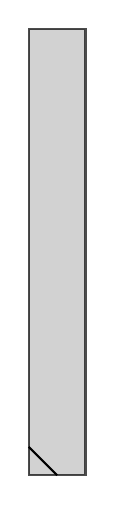
\begin{tikzpicture}[scale=1.5]
    \draw[fill=lightgray,opacity=0.7,thick] (0,0) rectangle (0.48,3.78);
    \draw[thick] (0,0.24) -- (0.24,0);
  \end{tikzpicture}
  \caption{Site \texttt{CoreSite}}
  \label{fig:coresite}
\end{figure}

\begin{lstlisting}[ basicstyle=\tt\small
                  , xleftmargin=25mm
                  , firstnumber=589
                  , numbers=left
                  , frame=l
                  , caption=Definition of the cell \texttt{sg13g2\_and2\_1} (\texttt{sg13g2\_stdcell.lef})
                  , label={lst:and2}
                  ]
MACRO sg13g2_and2_1
  CLASS CORE ;
  ORIGIN 0 0 ;
  FOREIGN sg13g2_and2_1 0 0 ;
  SIZE 2.4 BY 3.78 ;
  SYMMETRY X Y ;
  SITE CoreSite ;
  PIN A
    DIRECTION INPUT ;
    USE SIGNAL ;
    ANTENNAMODEL OXIDE1 ;
      ANTENNAGATEAREA 0.1924 LAYER Metal1 ;
    PORT
      LAYER Metal1 ;
        RECT 0.105 0.405 0.78 0.96 ;
    END
  END A
  PIN B
    DIRECTION INPUT ;
    USE SIGNAL ;
    ANTENNAMODEL OXIDE1 ;
      ANTENNAGATEAREA 0.1924 LAYER Metal1 ;
    PORT
      LAYER Metal1 ;
        RECT 0.78 1.435 1.17 1.87 ;
    END
  END B
  PIN X
    DIRECTION OUTPUT ;
    USE SIGNAL ;
    ANTENNADIFFAREA 0.6324 LAYER Metal1 ;
    PORT
      LAYER Metal1 ;
        RECT 1.775 2.14 2.275 3.11 ;
        RECT 2.04 0.78 2.275 3.11 ;
        RECT 1.775 0.78 2.275 1.36 ;
    END
  END X
  PIN VDD
    DIRECTION INOUT ;
    USE POWER ;
    SHAPE ABUTMENT ;
    NETEXPR "VDD VDD!" ;
    PORT
      LAYER Metal1 ;
        RECT 0 3.56 2.4 4 ;
        RECT 1.265 2.485 1.525 4 ;
        RECT 0.245 2.425 0.505 4 ;
    END
  END VDD
  PIN VSS
    DIRECTION INOUT ;
    USE GROUND ;
    SHAPE ABUTMENT ;
    NETEXPR "VSS VSS!" ;
    PORT
      LAYER Metal1 ;
        RECT 0 -0.22 2.4 0.22 ;
        RECT 1.265 -0.22 1.525 1.155 ;
    END
  END VSS
  OBS
    LAYER Metal1 ;
      RECT 0.755 2.05 1.015 3.11 ;
      RECT 0.245 2.05 1.56 2.24 ;
      RECT 1.4 1.57 1.56 2.24 ;
      RECT 0.245 1.14 0.505 2.24 ;
      RECT 1.4 1.57 1.74 1.9 ;
  END
  PROPERTY CatenaDesignType "deviceLevel" ;
END sg13g2_and2_1
\end{lstlisting}


\begin{figure}[H]
  \centering
  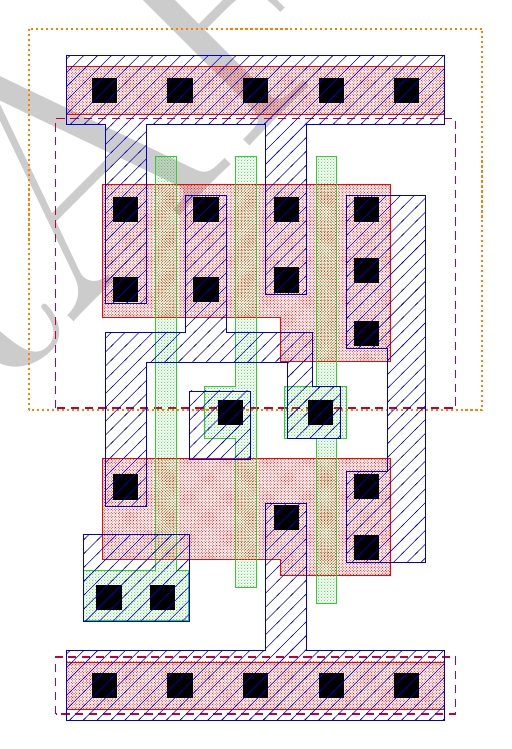
\begin{tikzpicture}[scale=2]

    \draw[NWell_drawing] (-0.24,1.75) rectangle (2.64,4.17);

    \draw[pSD_drawing] (-0.07,-0.18) rectangle (2.47,0.18);
    \draw[pSD_drawing] (-0.07,1.76) rectangle (2.47,3.6);

    % Activ
    \fill[Activ_drawing] (0,3.63) rectangle (2.4,3.93);
    \fill[Activ_drawing] (0,-0.15) rectangle (2.4,0.15);
    \fill[Activ_drawing] (1.355,2.06) -- 
            (1.355,2.34) -- 
            (0.225,2.34) -- 
            (0.225,3.18) -- 
            (2.055,3.18) -- 
            (2.055,2.06) -- cycle;
   \fill[Activ_drawing] (1.355,0.7) -- 
           (1.355,0.8) -- 
           (0.225,0.8) -- 
           (0.225,1.44) -- 
           (2.055,1.44) -- 
           (2.055,0.7) -- cycle;

  % Activ
  \fill[GatPoly_drawing] (0.105,0.41) -- 
           (0.105,0.73) -- 
           (0.565,0.73) -- 
           (0.565,3.36) -- 
           (0.695,3.36) -- 
           (0.695,0.73) -- 
           (0.775,0.73) -- 
           (0.775,0.41) -- cycle;

  \fill[GatPoly_drawing] (1.07500,0.62000) -- 
      (1.07500,1.57000) -- 
      (0.87500,1.57000) -- 
      (0.87500,1.90000) -- 
      (1.07500,1.90000) -- 
      (1.07500,3.36000) -- 
      (1.20500,3.36000) -- 
      (1.20500,0.62000) -- cycle;

  \fill[GatPoly_drawing] (1.58500,0.52000) -- 
      (1.58500,1.57000) -- 
      (1.38500,1.57000) -- 
      (1.38500,1.90000) -- 
      (1.58500,1.90000) -- 
      (1.58500,3.36000) -- 
      (1.71500,3.36000) -- 
      (1.71500,1.90000) -- 
      (1.77500,1.90000) -- 
      (1.77500,1.57000) -- 
      (1.71500,1.57000) -- 
      (1.71500,0.52000) -- cycle;

    \fill[black] (0.16,-0.08) rectangle (0.32,0.08);
    \fill[black] (0.64,-0.08) rectangle (0.8,0.08);
    \fill[black] (1.12,-0.08) rectangle (1.28,0.08);
    \fill[black] (1.6,-0.08) rectangle (1.76,0.08);
    \fill[black] (2.08,-0.08) rectangle (2.24,0.08);

    \fill[black] (0.16,3.7) rectangle (0.32,3.86);
    \fill[black] (0.64,3.7) rectangle (0.8,3.86);
    \fill[black] (1.12,3.7) rectangle (1.28,3.86);
    \fill[black] (1.6,3.7) rectangle (1.76,3.86);
    \fill[black] (2.08,3.7) rectangle (2.24,3.86);

    \fill[black] (0.19,0.48) rectangle (0.35,0.64);
    \fill[black] (0.53,0.48) rectangle (0.69,0.64);
    \fill[black] (0.295,1.18) rectangle (0.455,1.34);
    \fill[black] (1.315,0.985) rectangle (1.475,1.145);
    \fill[black] (1.825,0.795) rectangle (1.985,0.955);
    \fill[black] (1.825,1.185) rectangle (1.985,1.345);   
    \fill[black] (0.96,1.655) rectangle (1.12,1.815);   
    \fill[black] (1.53,1.655) rectangle (1.69,1.815);

    \fill[black] (0.295,2.435) rectangle (0.455,2.595);
    \fill[black] (0.295,2.94) rectangle (0.455,3.1);
    \fill[black] (0.805,2.435) rectangle (0.965,2.595);
    \fill[black] (0.805,2.94) rectangle (0.965,3.1);
    \fill[black] (1.315,2.495) rectangle (1.475,2.655);
    \fill[black] (1.315,2.94) rectangle (1.475,3.1);
    \fill[black] (1.825,2.155) rectangle (1.985,2.315);
    \fill[black] (1.825,2.555) rectangle (1.985,2.715);
    \fill[black] (1.825,2.94) rectangle (1.985,3.1);

    % A (MET1)
    \fill[Metal1_drawing_big] (0.105,0.405) rectangle (0.78,0.96);

    % B (MET1)
    \fill[Metal1_drawing_big] (0.78,1.435) rectangle (1.17,1.87);

    % X (MET1)
    \fill[Metal1_drawing_big] (1.77500,0.78000) -- 
                          (1.77500,1.36000) -- 
                          (2.04000,1.36000) -- 
                          (2.04000,2.14000) -- 
                          (1.77500,2.14000) -- 
                          (1.77500,3.11000) -- 
                          (2.27500,3.11000) -- 
                          (2.27500,0.78000) -- cycle;

    % VDD (MET1)
    \fill[Metal1_drawing_big] (0.24500,2.42500) -- 
                        (0.24500,3.56000) -- 
                        (0.00000,3.56000) -- 
                        (0.00000,4.00000) -- 
                        (2.40000,4.00000) -- 
                        (2.40000,3.56000) -- 
                        (1.52500,3.56000) -- 
                        (1.52500,2.48500) -- 
                        (1.26500,2.48500) -- 
                        (1.26500,3.56000) -- 
                        (0.50500,3.56000) -- 
                        (0.50500,2.42500) -- cycle;

    % VSS (MET1)
    \fill[Metal1_drawing_big] (0.00000,-0.22000) -- 
                          (0.00000,0.22000) -- 
                          (1.26500,0.22000) -- 
                          (1.26500,1.15500) -- 
                          (1.52500,1.15500) -- 
                          (1.52500,0.22000) -- 
                          (2.40000,0.22000) -- 
                          (2.40000,-0.22000) -- cycle;

    % Obstruction (MET1)
    \fill[Metal1_drawing_big] (0.24500,1.14000) -- 
                          (0.24500,2.24000) -- 
                          (0.75500,2.24000) -- 
                          (0.75500,3.11000) -- 
                          (1.01500,3.11000) -- 
                          (1.01500,2.24000) -- 
                          (1.56000,2.24000) -- 
                          (1.56000,1.90000) -- 
                          (1.74000,1.90000) -- 
                          (1.74000,1.57000) -- 
                          (1.40000,1.57000) -- 
                          (1.40000,2.05000) -- 
                          (0.50500,2.05000) -- 
                          (0.50500,1.14000) -- cycle;
  \end{tikzpicture}
  \caption{Layout of \texttt{sg13g2\_and2\_1}
  (\protect\tikz\protect\draw[Activ_drawing] (0,0) rectangle (0.25,0.25);~\texttt{Activ},
   \protect\tikz\protect\draw[GatPoly_drawing] (0,0) rectangle (0.25,0.25);~\texttt{GatPoly},
   \protect\tikz\protect\draw[NWell_drawing] (0,0) rectangle (0.25,0.25);~\texttt{NWell},
   \protect\tikz\protect\draw[pSD_drawing] (0,0) rectangle (0.25,0.25);~\texttt{pSD},
   \protect\tikz\protect\draw[Metal1_drawing_big] (0,0) rectangle (0.25,0.25);~\texttt{Metal1})}
  \label{fig:layout:and2}
\end{figure}




\printbibliography

\end{document}